% file: overview.tex

%%%%%%%%%%%%%%%
\begin{frame}{}
  \begin{center}
    \movie[showcontrols, width = 0.50\textwidth, height = 0.30\textwidth]
    {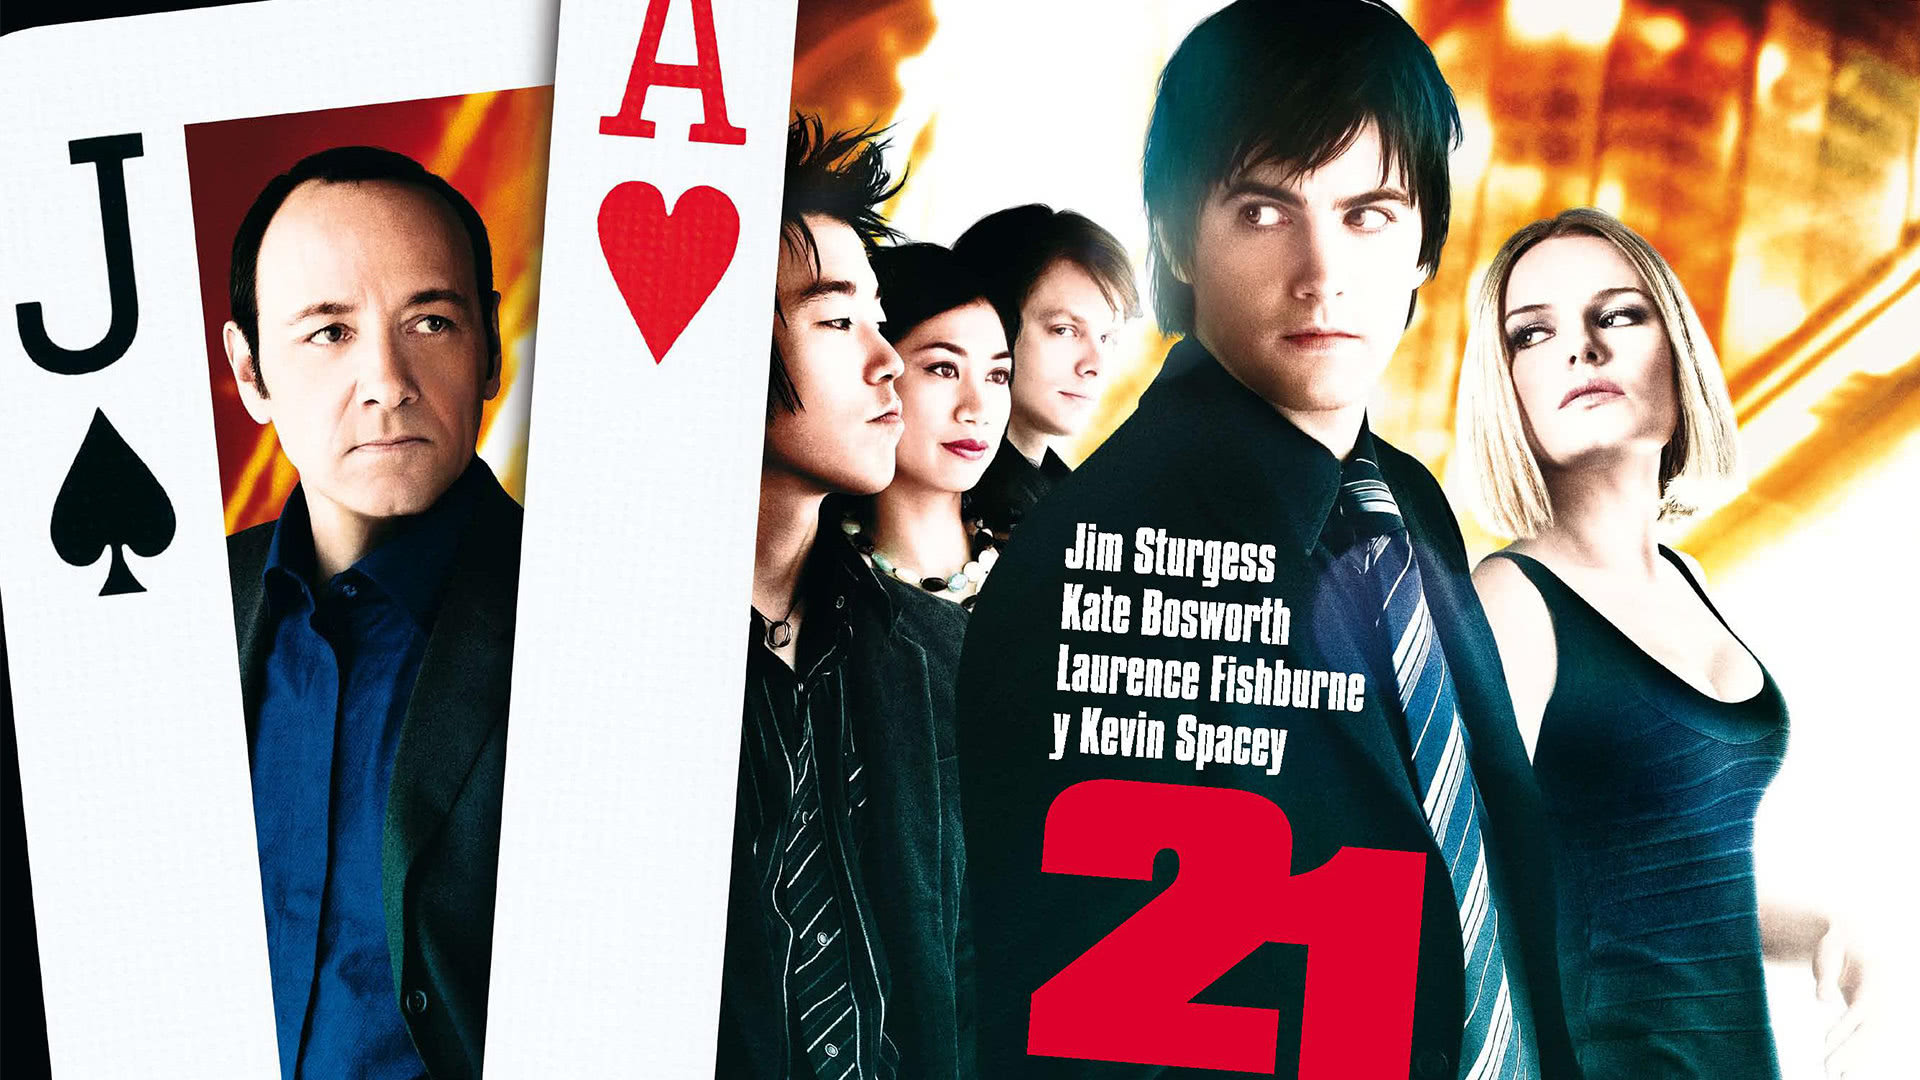
\includegraphics[width = 0.60\textwidth]{figs/21-film}}
    % \centerline{\begin{CJK*}{UTF8}{gbsn} 决胜 21 点 \end{CJK*}}
    {21-monty-hall.mp4}
  \end{center}
\end{frame}
%%%%%%%%%%%%%%%

%%%%%%%%%%%%%%%
\begin{frame}{}
  \begin{CJK*}{UTF8}{gbsn}
    \centerline{\teal{\LARGE 任务: 破坏与建设}}
  \end{CJK*}

  \pause
  \begin{columns}
    \column{0.50\textwidth}
      \fignocaption{width = 0.55\textwidth}{figs/chai}
    \column{0.50\textwidth}
      \pause
      \fignocaption{width = 0.85\textwidth}{figs/xiongan}
  \end{columns}
\end{frame}
%%%%%%%%%%%%%%%

%%%%%%%%%%%%%%%
\begin{frame}{}
  \begin{quote}
    ``\ldots and the many \purple{paradoxes} show clearly that we, as humans, 
    \purple{lack a well grounded intuition} in this matter.''

    \hfill --- {\small ``The Art of Probability'', Richard W. Hamming}
  \end{quote}

  \begin{columns}
    \column{0.50\textwidth}
      \fignocaption{width = 0.50\textwidth}{figs/intuition-told}
    \column{0.50\textwidth}
      \fignocaption{width = 0.70\textwidth}{figs/dice}
  \end{columns}

  \pause
  \vspace{0.50cm}
  \begin{quote}
    ``When called upon to judge probability, people actually judge something else
    and \textbf{\textit{\purple{believe}}} they have judged probability.''

    \hfill --- {\small ``Thinking, Fast and Slow'', Daniel Kahneman}
  \end{quote}
\end{frame}
%%%%%%%%%%%%%%%

%%%%%%%%%%%%%%%
% \begin{frame}{}
%   \fignocaption{width = 0.30\textwidth}{figs/Leibniz}
% 
%   \vspace{0.50cm}
%   \begin{quote}
%     \centerline{\red{\LARGE Let us calculate [calculemus].}}
%   \end{quote}
% \end{frame}
%%%%%%%%%%%%%%%
